\documentclass[a4paper]{article}

\usepackage[spanish]{babel}
\usepackage{graphicx}
\usepackage{amsmath, amssymb}
\usepackage[margin=2cm]{geometry}
\usepackage{fancyhdr}
\usepackage{enumerate}
\usepackage[shortlabels]{enumitem}
\usepackage{parskip}
\usepackage[most]{tcolorbox}
\usepackage[hidelinks]{hyperref}
\usepackage{float}
\usepackage{booktabs}



% cabecera
\pagestyle{fancy}
\fancyhead[l]{Astroestadística}
\fancyhead[c]{Tarea 1}
\fancyhead[r]{\today}
\fancyfoot[c]{\thepage}
\renewcommand{\headrulewidth}{0.2pt} % linea horizontal

\begin{document}

\begin{titlepage}
  \centering
  {\Large Universidad de Antioquia\par}
  \vspace{2cm}
  {\huge\bfseries Astroestadística\par}
  \vspace{0.4cm}
  {\Large Solución de la tarea \#1 \par}
  \vspace{2.5cm}
  {\large Autor:\par}
  \vspace{0.2cm}
  {\large Daniel Soto Villada\par}
  {\large Estudiante de Astronomía\par}
  \vfill
  {\large \today\par}
\end{titlepage}

\newpage
\tableofcontents
\newpage

\section{Problema \# 1}
\textbf{Enunciado:}
¿Qué es un histograma? Consulte y explique diferentes formas de construir un histograma según el número o tamaño de sus bines. ¿En qué casos se usan?

\subsection*{Solución}
Un \textbf{histograma} es un método de estadística descriptiva de naturaleza gráfica que permite resumir y describir las características importantes de un conjunto de datos numéricos. Visualmente, consiste en una serie de rectángulos verticales donde el área de cada uno es proporcional a la frecuencia relativa de los datos que representa.

Existen diferentes formas de construir un histograma dependiendo de la naturaleza de la variable y la disposición de sus intervalos o "bines":

\begin{enumerate}[a.]
    \item \textbf{Histograma para datos discretos:} Se utiliza cuando los datos resultan de un conteo. Se determina la frecuencia relativa de cada valor de la variable $x$ y se traza un rectángulo centrado sobre dicho valor, cuya altura es la frecuencia relativa.
    \item \textbf{Histograma para datos continuos con bines de ancho igual:} Se subdivide el eje de medición en intervalos de clase del mismo tamaño. El número de clases suele ser aproximadamente $\sqrt{n}$, donde $n$ es el número de observaciones. La altura de cada rectángulo es la frecuencia relativa de la clase.
    \item \textbf{Histograma para datos continuos con bines de ancho desigual (Escala de Densidad):} Se emplea cuando el conjunto de datos está 'alargado' hacia un lado o tiene valores extremos, donde bines de igual ancho dejarían muchas clases vacías o concentrarían todo en una sola. Aquí, la altura de los bines se denomina \textbf{densidad} y se calcula como:
    $$ \text{altura del rectángulo} = \frac{\text{frecuencia relativa de la clase}}{\text{ancho de la clase}} $$
    Esto garantiza que el área del rectángulo sea la frecuencia relativa y que el área total de todos los rectángulos sume 1.
\end{enumerate}

\textbf{Casos de uso:}
Los histogramas se usan para obtener una impresión preliminar de los datos, permitiendo identificar valores típicos, el grado de dispersión, la simetría (o asimetría), la presencia de brechas y el número de crestas (unimodal, bimodal o multimodal). El uso de bines desiguales es específico para casos con alta concentración de datos en una región y observaciones muy dispersas en otras.

\newpage

\section{Problema \# 2}
\textbf{Enunciado:}
Realice o simule el lanzamiento de dos dados de seis caras cada uno y guarde el resultado de la suma de los valores obtenidos. Repita el experimento un total de $n$ veces, con $n = 10, 100, 1000, 10000, 100000$.

\begin{enumerate}[a.]
    \item ¿Cuántas veces obtuvo cada resultado? Muestre sus resultados gráficamente para cada $n$. ¿Qué tipo de gráfico va a usar?
    \item ¿Cómo cambian los resultados a medida que $n$ aumenta?
    \item ¿Los resultados son los esperados? Explique.
    \item ¿Qué pasa cuando $n$ es muy grande? ¿Cómo interpretaría los resultados en términos de probabilidad?
\end{enumerate}

\subsection*{Solución}

\begin{figure}[H]
    \centering
    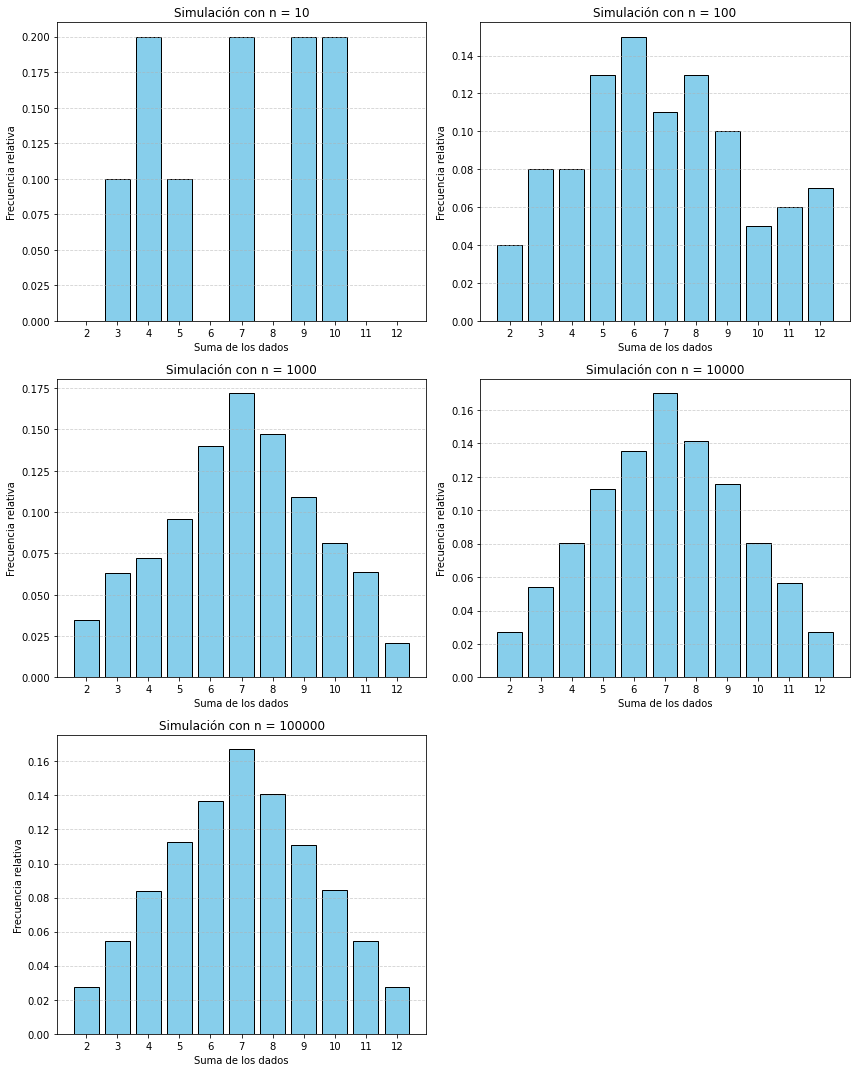
\includegraphics[width=0.75\textwidth]{HistogramasProblema2.png}
    \caption{Distribución de frecuencia relativa de la suma de dos dados de seis caras para diferentes tamaños de muestra ($n\in\{10,100,1000,10000,100000\})$}
    \label{fig:histograma}
\end{figure}

\begin{enumerate}[a.]
    \item Como se observa en la Figura 1, para $n=10$ la distribución es muy irregular y presenta brechas en valores posibles como el 2, 6, 7 y 8. Pero cuando $n$ crece, los bines se estabilizan.
    
    \item A medida que el tamaño de la muestra aumenta, el histograma se vuelve progresivamente más suave, simétrico y concentrado en torno a un valor central. Mientras que para $n=10$ y $n=100$ existen muchas irregularidades por la variabilidad del muestreo, en $n=10 000$ y $n=100 000$ la forma de la distribución se estabiliza bastante, mostrando una figura gaussiana con $\mu=7$.
    
    \item Los resultados son los esperados según la teoría de probabilidad para dados imparciales. Para dos dados, existen 36 resultados posibles en el espacio muestral. La suma con mayor probabilidad es el 7, ya que cuenta con 6 combinaciones favorables: (1,6), (2,5), (3,4), (4,3), (5,2) y (6,1), lo que equivale a $P(7) = 6/36 \approx 0.1667$. Las sumas de los extremos (2 y 12) son las menos probables con una frecuencia teórica de $1/36 \approx 0.0278$. Los histogramas de $n=100000$ reflejan casi exactamente estas proporciones teóricas.
    
    \item Cuando $n$ es muy grande, la frecuencia relativa observada de cada suma tiende a un valor límite. Esto significa que la probabilidad de un evento (como obtener una suma de 7) es la proporción de veces que ocurrirá dicho evento en una secuencia interminable de ensayos idénticos e independientes. El hecho de que el histograma se estabilice en una forma definida al aumentar $n$ demuestra empíricamente cómo la incertidumbre individual se convierte en una regularidad estadística.
\end{enumerate}


\section{Problema \# 3}
\textbf{Enunciado:}
Haga un análisis bien fundamentado (y en la medida de las posibilidades, basado en evidencia) que le permita, a través de sus priors, asignar una probabilidad subjetiva al evento de aprobar el curso de astroestadística. Argumente su respuesta.

\subsection*{Solución}

El \textbf{prior} o probabilidad inicial ($P(A)$) se establece en un $50\%$,se fundamenta en la evidencia histórica de que usualmente apruebo la mitad de mis materias cursadas.

Al transcurrir el primer $15\%$ del curso aproximadamente, obserbo desde dos perspectivas: \textbf{Evidencia negativa:} Desempeño deficiente en las primeras clases y tareas. \textbf{Evidencia positiva:} dedico 6 horas semanales al estudio de este curso, me gusta la estadística y estoy mejorando mi estado de salud.

Ahora podemos calcular una \textbf{probabilidad posterior} ($P(A|B)$). A pesar del inicio difícil (debido a problemas de salud críticos), el aumento en el tiempo de estudio, la mejoría en la salud y el ánimo para aprender, actúan como factores que reducen la incertidumbrey inicial. La nueva \textbf{probabilidad subjetiva} asignada al evento de aprobar es del $90\%$


\bibliographystyle{plainurl}
\bibliography{bibliografia} 
\end{document}
